%
% ground_segment.tex
%
% Copyright The Radio Occultation Contributors.
%
% Radio Occultation Documentation
%
% This work is licensed under the Creative Commons Attribution-ShareAlike 4.0
% International License. To view a copy of this license,
% visit http://creativecommons.org/licenses/by-sa/4.0/.
%

%
% \brief Ground segment chapter.
%
% \author Gabriel Mariano Marcelino <gabriel.mm8@gmail.com>
%
% \version 0.2.0
%
% \date 2020/06/06
%

\chapter{ \textcolor{red}{TODO} Ground Segment} \label{ch:ground-segment}

This chapter describes the ground segment of the mission. It is composed of two ground stations (one at the INPE-RN installations and the other at the SpaceLab installations) and many data collection platforms (PCD\nomenclature{\textbf{PCD}}{\textit{``Plataforma de Coleta de Dados'', or Data Collection Platform}}, or \textit{``Plataforma de Coleta de Dados''}), installed at a variety of locations on the Brazilian territory.

The control of the mission and the reception of the collected data will be performed mainly at these two ground stations, but if necessary, other stations can execute this task. Any station in the world can use the amateur radio link since having the required equipment to it.

\section{ \textcolor{red}{TODO} UFSC Ground Station}

The UFSC ground station is currently being developed and prepared for this mission. This section presents the project of this station. A general block diagram can be seen in \autoref{fig:grs-block-diagram}.

\begin{figure}[!ht]
    \begin{center}
        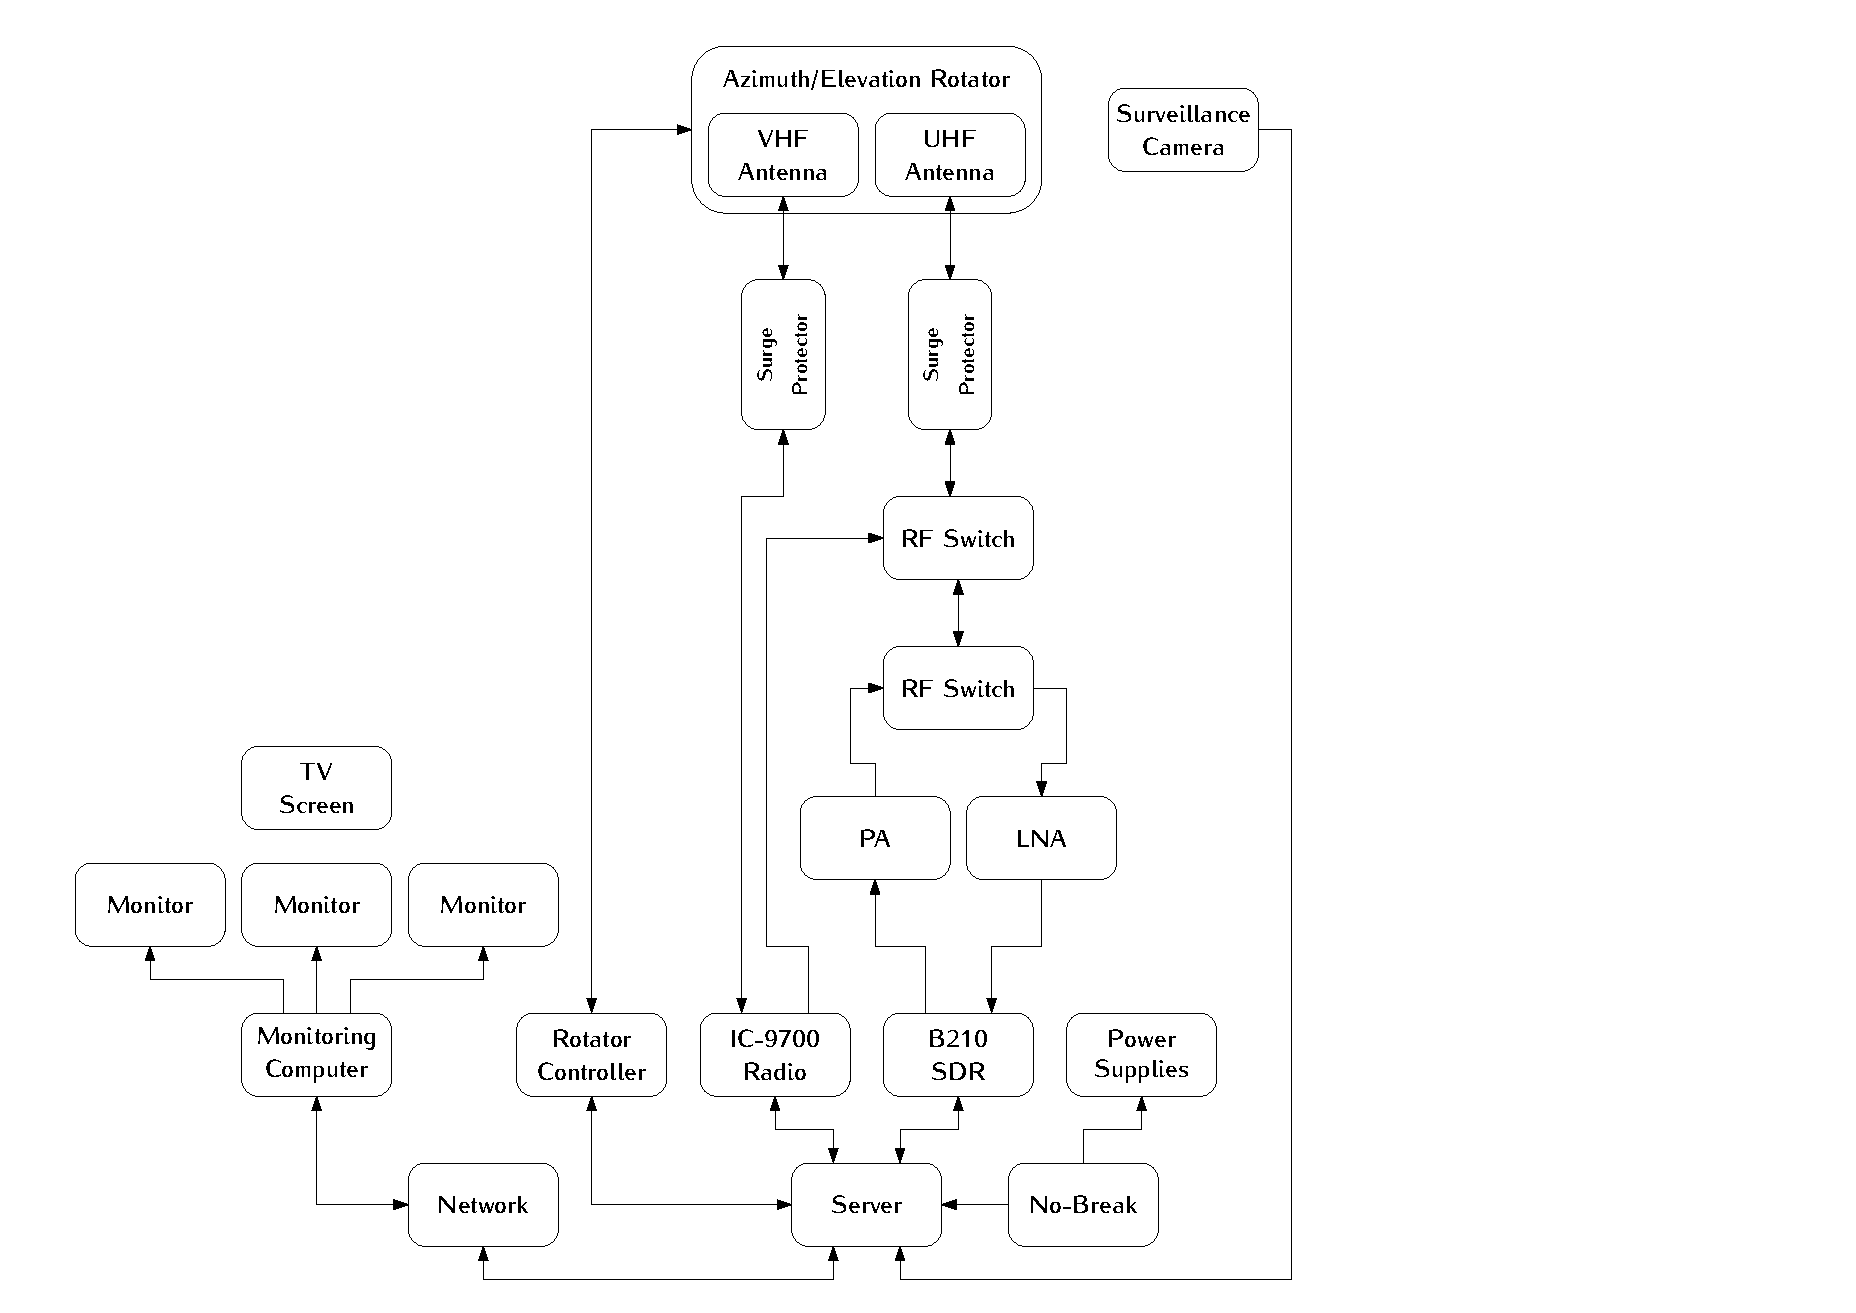
\includegraphics[width=\textwidth]{figures/grs-block-diagram.pdf}
        \caption{Block diagram of the ground segment (UFSC ground station).}
        \label{fig:grs-block-diagram}
    \end{center}
\end{figure}

In the following sections, a description of the main components of the station will be presented.

\subsection{ \textcolor{red}{TODO} Hardware}

This part describes the hardware side of the UFSC ground station and details the main peripherals that will be used in this project. Most of the components described here are represented in \autoref{fig:grs-block-diagram}.

\subsubsection{Antennas}

There are two antennas in the ground station: One for VHF and one for the UHF band. The main characteristics of these antennas can be seen in \autoref{tab:grs-antennas}

\begin{table}[ht]
    \centering
    \begin{tabular}{lccc}
        \toprule[1.5pt]
        \textbf{Characteristic} & \textbf{VHF Antenna}  & \textbf{UHF Antenna}  & \textbf{Unit} \\
        \midrule
        Brand                   & M$^{2}$               & Cushcraft             & - \\
        Model                   & 2MCP14                & A719B                 & - \\
        Type                    & Yagi                  & Yagi                  & - \\
        Number of elements      & 14                    & 19                    & - \\
        Frequency range         & 143-148               & 430-450               & MHz \\
        Gain                    & 12.34                 & 15.5                  & dBi \\
        Power rating            & 1500                  & 2000                  & W \\
        Boom length             & 3.2                   & 4.1                   & m \\
        Longest element         & 1.02                  & 0.34                  & m \\
        Weight                  & 2.72                  & 2.55                  & kg \\
        \bottomrule[1.5pt]
    \end{tabular}
    \caption{Main characteristics of the ground segment antennas.}
    \label{tab:grs-antennas}
\end{table}

More information about the VHF and UHF antennas can be found in \cite{2mcp14} and \cite{a719b} respectively.

\paragraph{Surge Protector}

Two surge protectors will be used to protect the ground station electronics of possible atmospheric discharges in the outside components (one for each antenna). The gas surge protectors safely discharge/deflect up to 5000 A of peak current to earth without causing damage to an independent ground. This device is installed near the antennas, in cascade with the RF cables.

For this project, the model MFJ-270N will be used, and a picture of it can be seen in \autoref{fig:mfj-270n}.

\begin{figure}[!ht]
    \begin{center}
        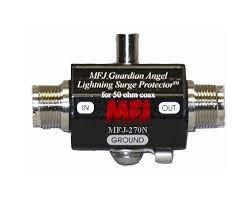
\includegraphics[width=0.4\textwidth]{figures/mfj-270n.jpeg}
        \caption{MFJ-270N surge protector.}
        \label{fig:mfj-270n}
    \end{center}
\end{figure}

\subsubsection{Rotators}

Both antennas (VHF and UHF) track the satellite through a two axis rotator (azimuth and elevation). The used model is the Yaesu G-5500, which provides 450$^{\circ}$ azimuth and 180$^{\circ}$ elevation control of medium and large size unidirectional satellite antenna arrays under remote control from station operation position.

A picture of the G-5500 rotator (and controller) can be seen in \autoref{fig:g5500}; the main characteristics can be found in \autoref{tab:grs-rotor}.

\begin{figure}[!ht]
    \begin{center}
        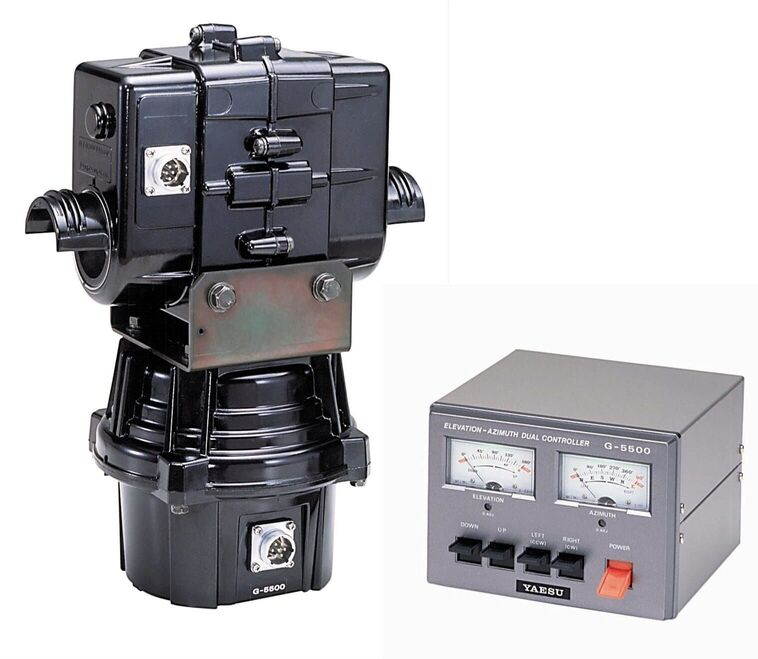
\includegraphics[width=0.6\textwidth]{figures/g5500.jpg}
        \caption{Yaesu G-5500 rotator and controller.}
        \label{fig:g5500}
    \end{center}
\end{figure}

\begin{table}[ht]
    \centering
    \begin{tabular}{lcc}
        \toprule[1.5pt]
        \textbf{Characteristic}                     & \textbf{Value}        & \textbf{Unit} \\
        \midrule
        Brand                                       & Yaesu                 & - \\
        Model                                       & G-5500                & - \\
        Voltage requirement                         & 110-120 or 200-240    & $V_{AC}$ \\
        Motor voltage                               & 24                    & V$_{AC}$ \\
        Rotation time (elevation, 180$^{\circ}$)    & 67                    & s \\
        Rotation time (azimuth, 360$^{\circ}$)      & 58                    & s \\
        Maximum continuous operation                & 5                     & min \\
        Rotation torque (elevation)                 & 14                    & kg-m \\
        Rotation torque (azimuth)                   & 6                     & kg-m \\
        Braking torque (elevation and azimuth)      & 40                    & kg-m \\
        Vertical load                               & 200                   & kg \\
        Pointing accuracy                           & $\pm$ 4               & \% \\
        Wind surface area                           & 1                     & $m^{2}$ \\
        Weight (rotator)                            & 9                     & kg \\
        Weight (controller)                         & 3                     & kg \\
        \bottomrule[1.5pt]
    \end{tabular}
    \caption{Main characteristics of antennas' rotators.}
    \label{tab:grs-rotor}
\end{table}

More information about the ground station rotator can be found in \cite{g5500}.

\subsubsection{Amplifiers}

There are two dedicated amplifiers in the UFSC ground station: one power amplifier (PA) for transmitting telecommands with a high power signal, and a low noise amplifier (LNA), for amplify the received signals from the satellite. Both are presented next.

\paragraph{Power Amplifier}

The power amplifier is used to add a gain to the generated signals of the transmitter. The used model is the Mini-Circuits ZHL-50W-52-S+ \cite{zhl50w}. A picture of this power amplifier can be seen in \autoref{fig:zhl-50w}, the main characteristics are available in \autoref{tab:zhl-50w-specs}.

\begin{figure}[!ht]
    \begin{center}
        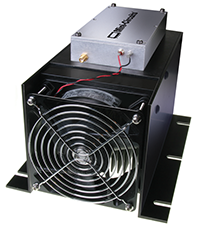
\includegraphics[width=0.3\textwidth]{figures/zhl-50w.png}
        \caption{Mini-Circuits ZHL-50W-52-S+ power amplifier.}
        \label{fig:zhl-50w}
    \end{center}
\end{figure}

\begin{table}[ht]
    \centering
    \begin{tabular}{lcc}
        \toprule[1.5pt]
        \textbf{Characteristic} & \textbf{Value}    & \textbf{Unit} \\
        \midrule
        Brand                   & Mini-Circuits     & - \\
        Model                   & ZHL-50W-52-S+     & - \\
        Frequency range         & 50-500            & MHz \\
        Gain                    & 47-52             & dB \\
        Noise figure            & 4.5-7.0           & dB \\
        DC supply voltage       & 24-25             & V \\
        Max. supply current     & 9.3               & A \\
        \bottomrule[1.5pt]
    \end{tabular}
    \caption{Main characteristics of the ZHL-50W-52-S+ power amplifier.}
    \label{tab:zhl-50w-specs}
\end{table}

\paragraph{Low Noise Amplifiers}

As LNA, the model ZFL-500LN+ from Mini-Circuits \cite{zfl500ln} is being used. This amplifier will be used just after the antennas to add a gain to the incoming telemetry signals transmitted by the satellite. A picture of the low noise amplifier can be seen in \autoref{fig:lna}, the main characteristics are available in \autoref{tab:lna-specs}.

\begin{figure}[!ht]
    \begin{center}
        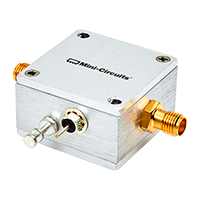
\includegraphics[width=150pt]{figures/lna.png}
        \caption{Mini-Circuits ZFL-500LN+ low noise amplifier.}
        \label{fig:lna}
    \end{center}
\end{figure}

\begin{table}[ht]
    \centering
    \begin{tabular}{lcc}
        \toprule[1.5pt]
        \textbf{Characteristic} & \textbf{Value}    & \textbf{Unit} \\
        \midrule
        Brand                   & Mini-Circuits     & - \\
        Model                   & ZFL-500LN+        & - \\
        Frequency range         & 0.1-500           & MHz \\
        Gain                    & 24-28             & dB \\
        DC supply voltage       & 15                & V \\
        Max. supply current     & 60                & mA \\
        \bottomrule[1.5pt]
    \end{tabular}
    \caption{Main characteristics of the ZFL-500LN+ low noise amplifier.}
    \label{tab:lna-specs}
\end{table}

\subsubsection{Radios}

Besides the SDR solution presented in the block diagram of the \autoref{fig:grs-block-diagram}, there is also a amateur radio transceiver with a standalone solution for the amateur radio link with the satellite. The used model is the Icom IC-9700 \cite{ic9700}, that is an RF direct sampling receiver for 2 m and 70 cm. The IF receiver consists of a single down conversion for 23 cm that is between 311 and 371 MHz. The PA provides 100 W on 2 m, 75 W on 70 cm, and 10 W on 23 cm.

In addition to band-specific memory channels, the IC-9700 allows the band-specific receiver and transmitter settings. For transmission, users can adjust RF power, TX power Limit, Limit Power, and TX Delay by the band. Basic receiver settings, like the Noise Blanker, Noise Reduction, and others, can be tweaked by the band with a dynamic Notch and Filter setup by band/mode. A picture of the IC-9700 radio can be seen in \autoref{fig:ic9700}.

\begin{figure}[!ht]
    \begin{center}
        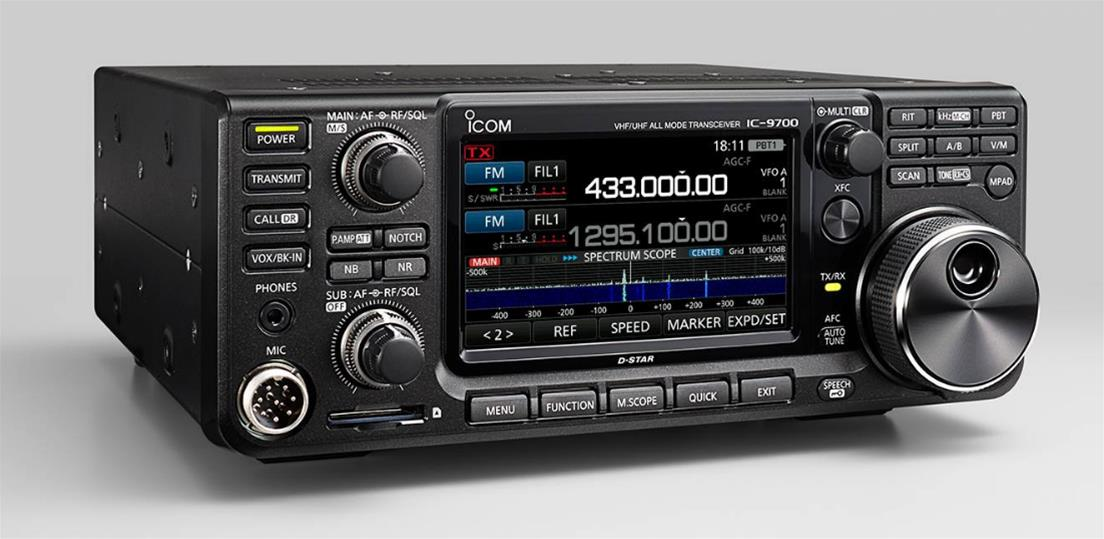
\includegraphics[width=0.7\textwidth]{figures/ic-9700.jpg}
        \caption{Icom IC-9700 radio transceiver.}
        \label{fig:ic9700}
    \end{center}
\end{figure}

\paragraph{Software Defined Radio}

As presented in \autoref{fig:grs-block-diagram}, the ground segment also has an SDR\nomenclature{\textbf{SDR}}{\textit{Software Defined Radio.}} (Software Defined Radio) as a transceiver. The used model is the USRP B210, from Ettus Research \cite{b210}, a fully integrated, single-board SDR with continuous frequency coverage from 70 MHz to 6 GHz. It combines the AD9361 RFIC direct-conversion transceiver providing up to 56 MHz of real-time bandwidth, an open and reprogrammable Spartan6 FPGA, and USB 3.0 connectivity. Also, full support for the USRP Hardware Driver (UHD) software allows the use of the GNURadio framework. A picture of the USRP B210 SDR (with enclosure) can be seen in \autoref{fig:usrp-b210}.

\begin{figure}[!ht]
    \begin{center}
        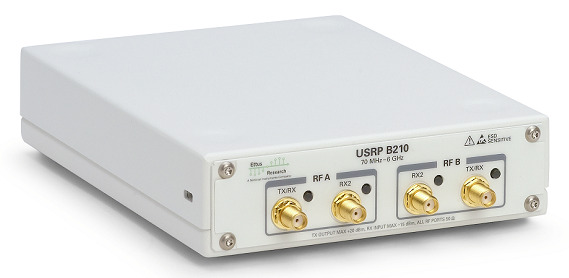
\includegraphics[width=0.6\textwidth]{figures/usrp-b210.jpg}
        \caption{Ettus USRP B210 SDR.}
        \label{fig:usrp-b210}
    \end{center}
\end{figure}

\subsubsection{Processing and Control}

The ground station control room shall have two monitors and a dedicated computer alongside most of the previously presented hardware. It will work as a monitoring room with a nobreak to protect the equipment from power grid fluctuations. 

The antennas and rotator will also be monitored with outside cameras. And the room will count with a server so that the transmission and decoding can be done remotely and at any time.

In the \autoref{fig:server} can be seen a picture of the used server, and in \autoref{tab:server} are presented the main characteristics of the it.

\begin{table}[ht]
    \centering
    \begin{tabular}{lc}
        \toprule[1.5pt]
        \textbf{Characteristic} & \textbf{Value} \\
        \midrule
        Brand                   & Dell \\
        Model                   & PowerEdge R240 \\
        Processor               & Intel Xeon E-2244G 3.8 GHz 4C/8T \\
        RAM Memory              & 16 GB DDR4 ECC \\
        Storage                 & 1 TB HD \\
        \bottomrule[1.5pt]
    \end{tabular}
    \caption{Main characteristics of the Dell PowerEdge R240 server.}
    \label{tab:server}
\end{table}

\begin{figure}[!ht]
    \begin{center}
        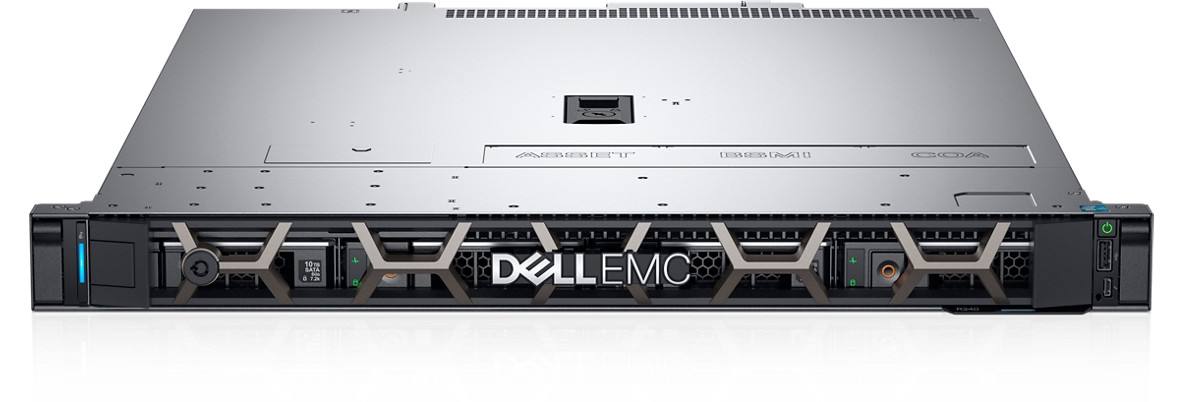
\includegraphics[width=300pt]{figures/server.jpg}
        \caption{Dell PowerEdge R240 server.}
        \label{fig:server}
    \end{center}
\end{figure}

\subsection{ \textcolor{red}{TODO} Satellite Tracking}

To track the satellite and for orbit prediction, the GPredict software \cite{gpredict} will be used. Gpredict is a real-time satellite tracking and orbit prediction application. It can track many satellites and display their position and other data in lists, tables, maps, and polar plots (radar view). Gpredict can also predict the time of future passes for a satellite and provide detailed information about each pass. Gpredict is free software licensed under the GNU General Public License. A picture of the main window of GPredict can be seen in \autoref{fig:gpredict}.

\begin{figure}[!ht]
    \begin{center}
        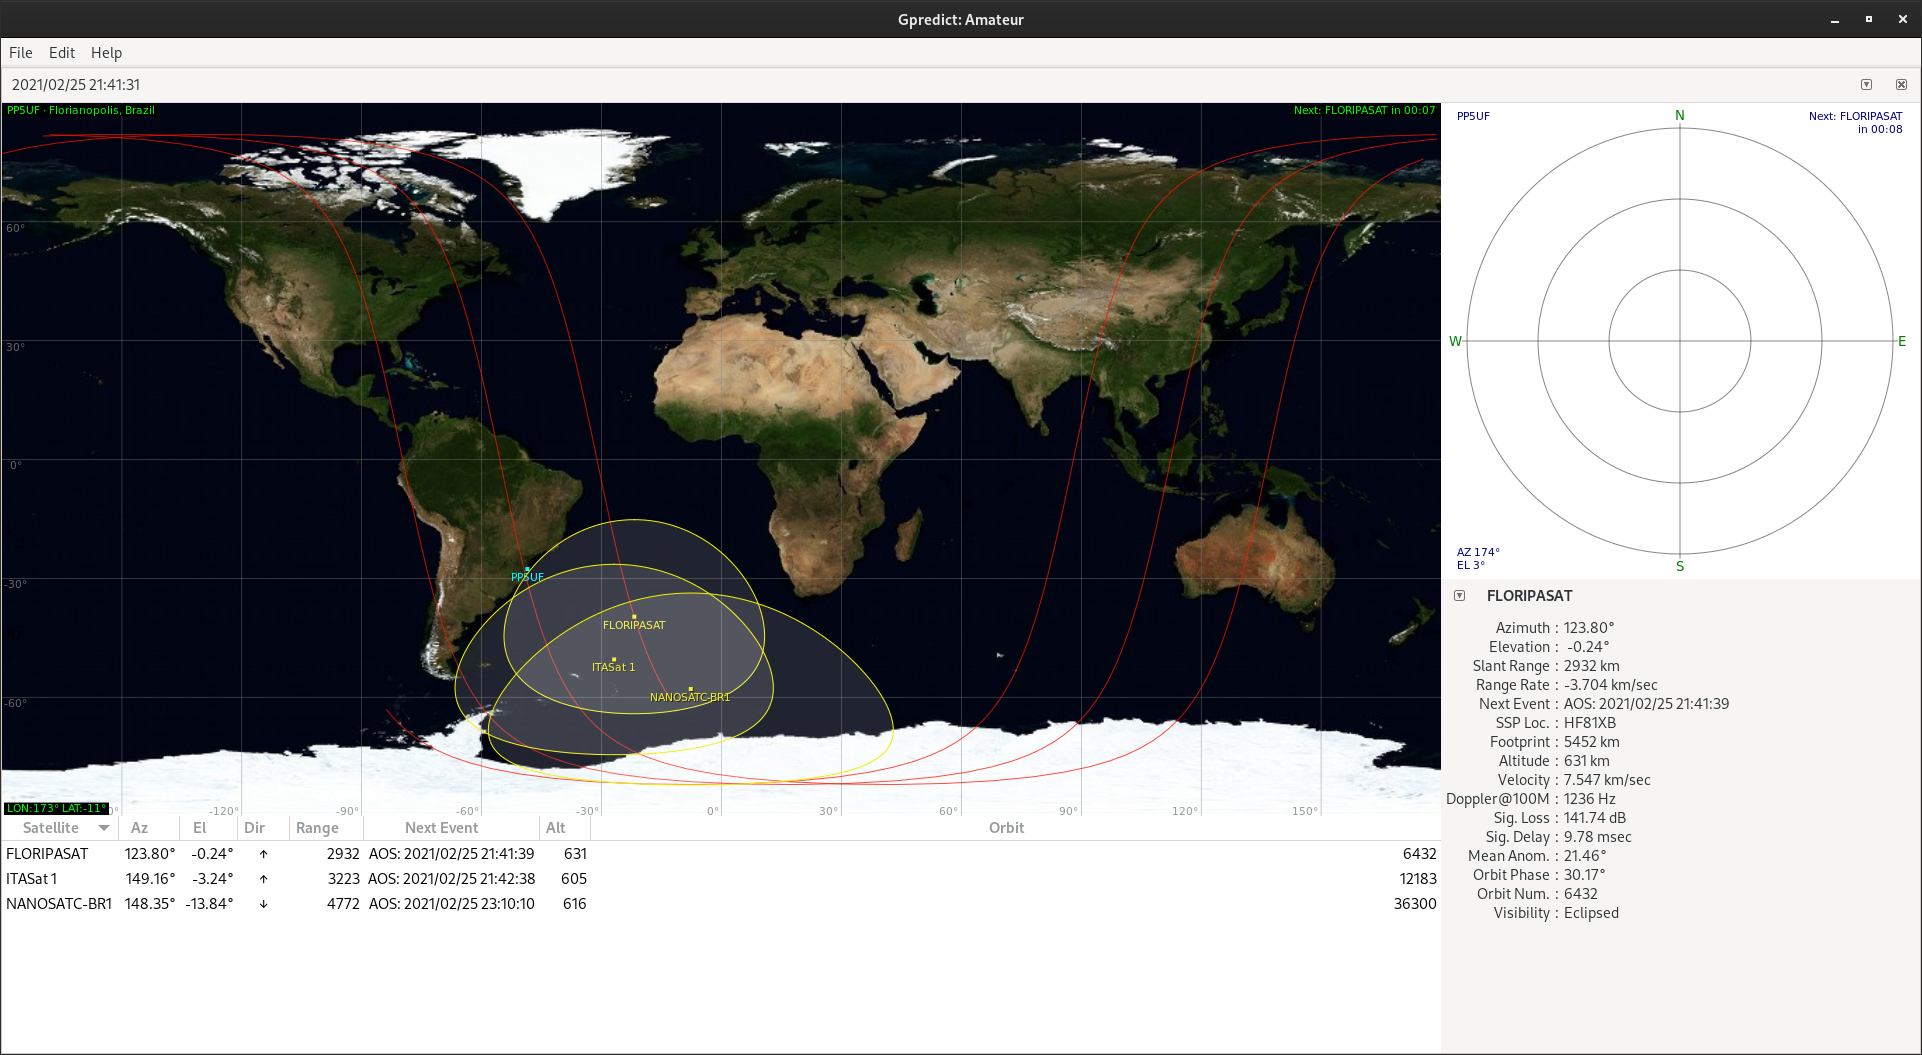
\includegraphics[width=\textwidth]{figures/gpredict.png}
        \caption{Main window of GPredict.}
        \label{fig:gpredict}
    \end{center}
\end{figure}

\subsection{ \textcolor{red}{TODO} Packet Transmission}

The packet generation and transmission to Radio Occultation satellite can be done with the SpaceLab-Transmitter software \cite{spacelab-transmitter}, which was written in Python with the interface developed using the GTK framework. It has a USRP Handler made with Ettus libraries to work with Ettus USRP B210 as shown in \autoref{fig:usrp-b210}. The supported modulation is the Gaussian Minimum Shift Keying (GMSK). Furthermore, the software also has unit tests for the main modules and a logging system to record events such as an initialization or a successfully transmitted telecommand.

In the \autoref{fig:transmitter-tree} is shown the product tree of the software, which contains its main elements of it, and in the \autoref{fig:spacelab-transmitter} is shown the main window of it.

\begin{figure}[!ht]
    \begin{center}
        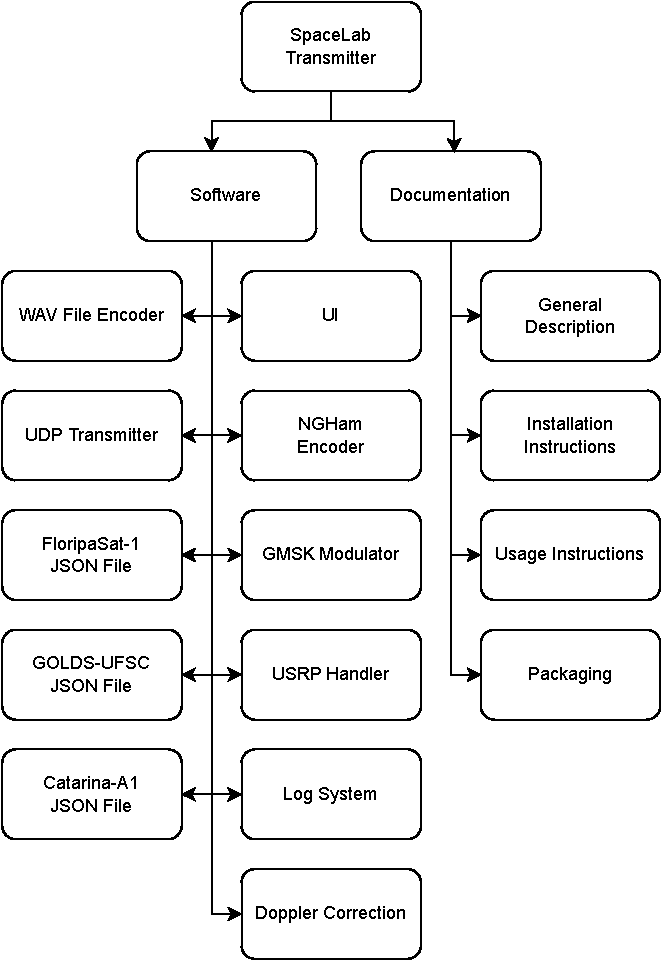
\includegraphics[width=0.6\textwidth]{figures/transmitter_tree.pdf}
        \caption{SpaceLab-Transmitter product tree.}
        \label{fig:transmitter-tree}
    \end{center}
\end{figure}

\begin{figure}[!ht]
    \begin{center}
        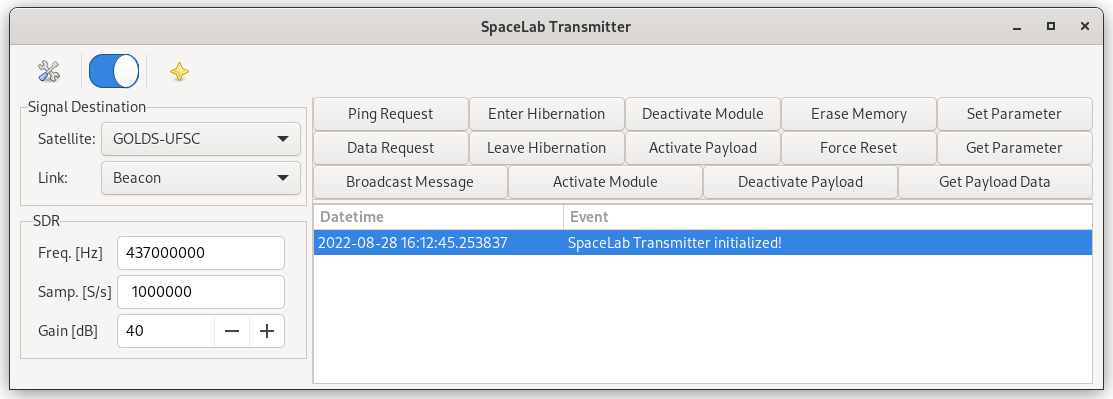
\includegraphics[width=\textwidth]{figures/spacelab-transmitter-window.png}
        \caption{Main window of the SpaceLab-Transmitter application.}
        \label{fig:spacelab-transmitter}
    \end{center}
\end{figure}

\subsection{ \textcolor{red}{TODO} Packet Decoding}

The packet decoding of Radio Occultation satellites telemetry can be done using the SpaceLab-Decoder \cite{spacelab-decoder} software using a .wav file or through a real time reception. The decoded telemetry will appear in a dialog within the main window. The software was written in Python, and the interface was developed using GTK framework. Furthermore, the software also has unit tests for the main modules and a logging system to record events.

The \autoref{fig:decoder-tree} is showing the product tree of the software, which contains its main elements, and in the \autoref{fig:spacelab-transmitter} is shown the main window of it.

\begin{figure}[!ht]
    \begin{center}
        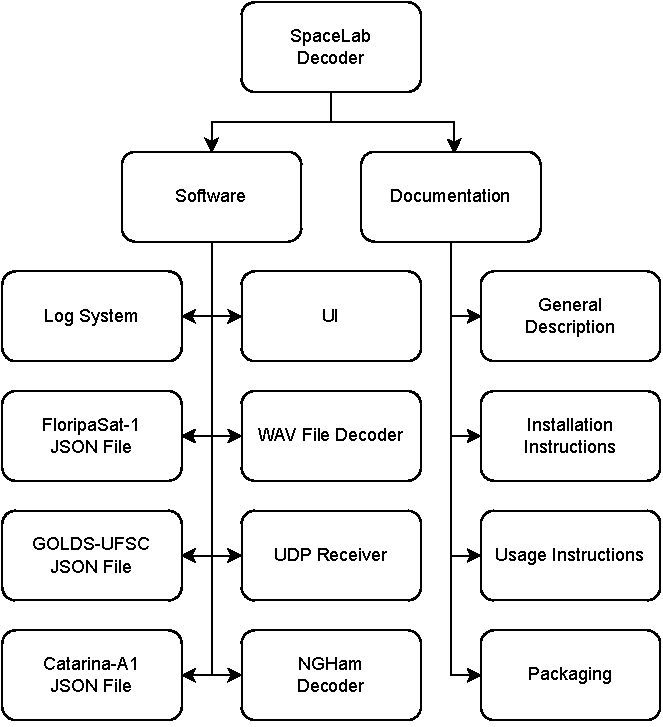
\includegraphics[width=0.6\textwidth]{figures/decoder_tree.pdf}
        \caption{SpaceLab-Decoder product tree.}
        \label{fig:decoder-tree}
    \end{center}
\end{figure}

\begin{figure}[!ht]
    \begin{center}
        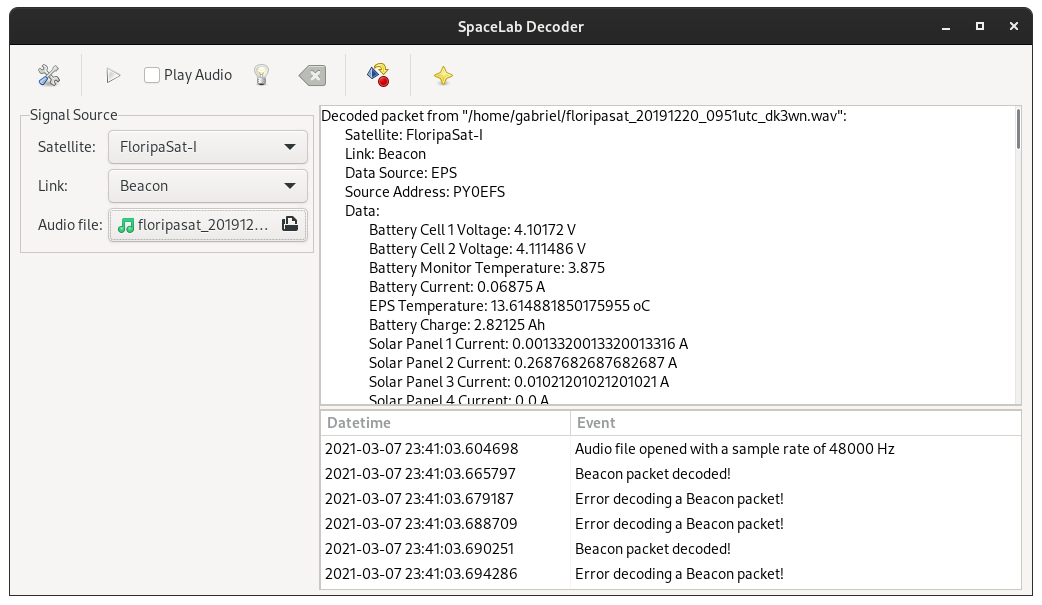
\includegraphics[width=\textwidth]{figures/spacelab-decoder.png}
        \caption{Main window of the SpaceLab-Decoder application.}
        \label{fig:spacelab-decoder}
    \end{center}
\end{figure}

\section{ \textcolor{red}{TODO} EMMN Ground Station}

The EMMN\nomenclature{\textbf{EMMN}}{\textit{Estação Mutlimissão de Natal.}} (\textit{Estação Multimissão de Natal} in portuguese) ground station \cite{emmn} was designed to operate in VHF, UHF and S-Band frequency bands, receiving payload and telemetry data and transmitting telecommands from and to satellites operating in low orbits.

The station's radio frequency systems use Software Defined Radios (SDRs), which offer the flexibility to quickly reconfigure parameters such as modulation type, encoding, datarate, etc. Most commonly used modulation schemes and encoding methods are already implemented, and any customization requests can be requested.

The station performs autonomous tracking of several satellites according to a previous schedule and a scale of priorities. A Client-Server network design allows station users to send and receive data remotely.

A general block diagram of the EMMN hardware is available in \autoref{fig:emmn-bd}.

\begin{figure}[!ht]
    \begin{center}
        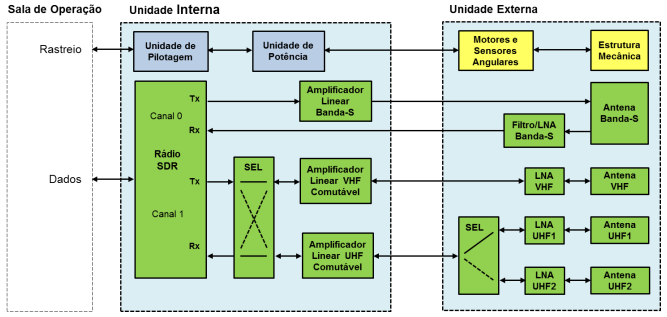
\includegraphics[width=\textwidth]{figures/emmn-bd}
        \caption{General block diagram of the EMMN.}
        \label{fig:emmn-bd}
    \end{center}
\end{figure}

\begin{table}[!h]
    \centering
    \begin{tabular}{lC{6cm}}
        \toprule[1.5pt]
        \textbf{Parameter} & \textbf{Value} \\
        \midrule
        Grid locator    & HI24JD59CI \\
        Coordinates     & -5.835238, -35.209285 \\
        Altitude        & 51 m \\
        Antennas        & Yagi and parabolic \\
        Bands           & VHF, UHF and S-Band\\
        Frequencies     & 144-146 MHz (VHF), 395-405 and 432-440 MHz (UHF) 2200-3300 MHz (S-Band)\\
        \bottomrule[1.5pt]
    \end{tabular}
    \caption{EMMN specs.}
    \label{tab:emmn-info}
\end{table}

\begin{figure}[!ht]
    \begin{center}
        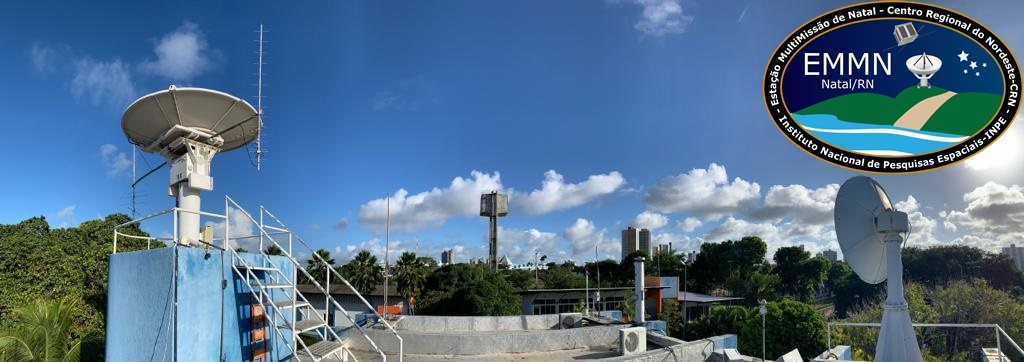
\includegraphics[width=\textwidth]{figures/inpe-emmn}
        \caption{Multimission station of Natal-RN.}
        \label{fig:emmn}
    \end{center}
\end{figure}

\section{ \textcolor{red}{TODO} Data Collection Platforms}

Data Collection Platforms (DCPs) are part of the Integrated System of Environmental Data (\textit{Sistema Integrado de Dados Ambientais, SINDA} \cite{sinda}, in Portuguese), which collects the data and by satellites, it is retransmitted to be received in the ground station so that it can be sent to SINDA to be processed. The data is shown online sometime after the receiving. Examples of DCPs can be seen in \autoref{fig:dcp-ex}.

\begin{figure}[!htb]
    \begin{center}
        \subfigure[\label{fig:dcp-ex-1}]{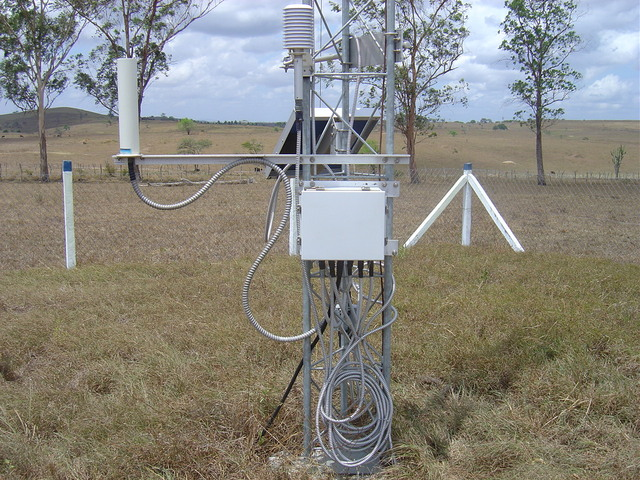
\includegraphics[width=0.48\textwidth]{figures/pcd-1}}
        ~
        \subfigure[\label{fig:dcp-ex-2}]{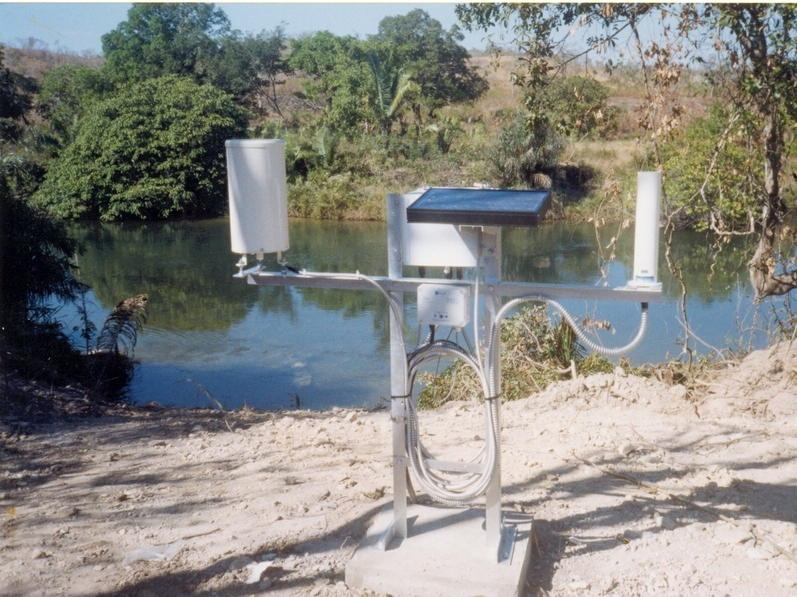
\includegraphics[width=0.48\textwidth]{figures/pcd-2}}

        \subfigure[\label{fig:dcp-ex-2}]{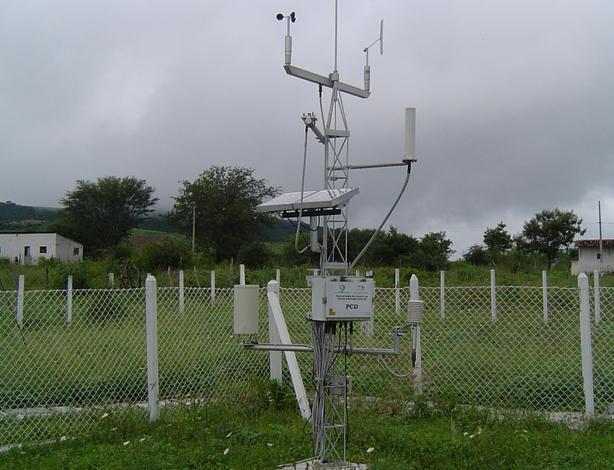
\includegraphics[width=0.48\textwidth]{figures/pcd-3}}
        \caption{Examples of data collection platforms (DCPs).}
        \label{fig:dcp-ex}
    \end{center}
\end{figure}
